\newcommand{\matlab}{MATLAB\textsuperscript{\textregistered}}
\chapter{What is \pharmml?}
\label{chap:pharmml-what}

\section{The Problem}\index{PharmML} 

The principal problem that \pharmml addresses is the reliable exchange of pharmacometric 
models between software tools. This is illustrated in Figure \ref{fig:platformDDMoRe}, where 
\pharmml is the exchange medium
for pharmacometric models for the main modelling and simulation tools in the field. This goal
has been successfully realised in the field of systems biology, neurobiology or data mining.

In systems biology for example software tools exchange models using the Systems Biology Markup 
Language \index{SBML}(SBML; \url{http://www.sbml.org}) \cite{SBML} and many published models can 
be found in the BioModels Database (\url{http://www.ebi.ac.uk/biomodels-main/}) 
\cite{BioModels2010}\index{BioModels}. Modellers don't worry about the
content of an SBML file; they rely on the fact that when they exchange it between the
modelling tools, it just works. Crucial to its success has been an active community of tool
developers and modellers who have supported and used it during
that time. Equally important has been the provision of sophisticated software libraries (libSBML
and JSBML) that take away much of the pain a software tool developer would otherwise experience
supporting what is now quite a complex standard. It is a virtuous circle. Users demand their
modelling tools support SBML\@. Developers provide reliable SBML support using libSBML, which
enables them to give their users what they want. The more tools that support SBML, the more useful
it becomes. The cost of supporting SBML is not negligible but quality libraries like libSBML make
the cost acceptable.

\begin{figure}[htb]
\centering
  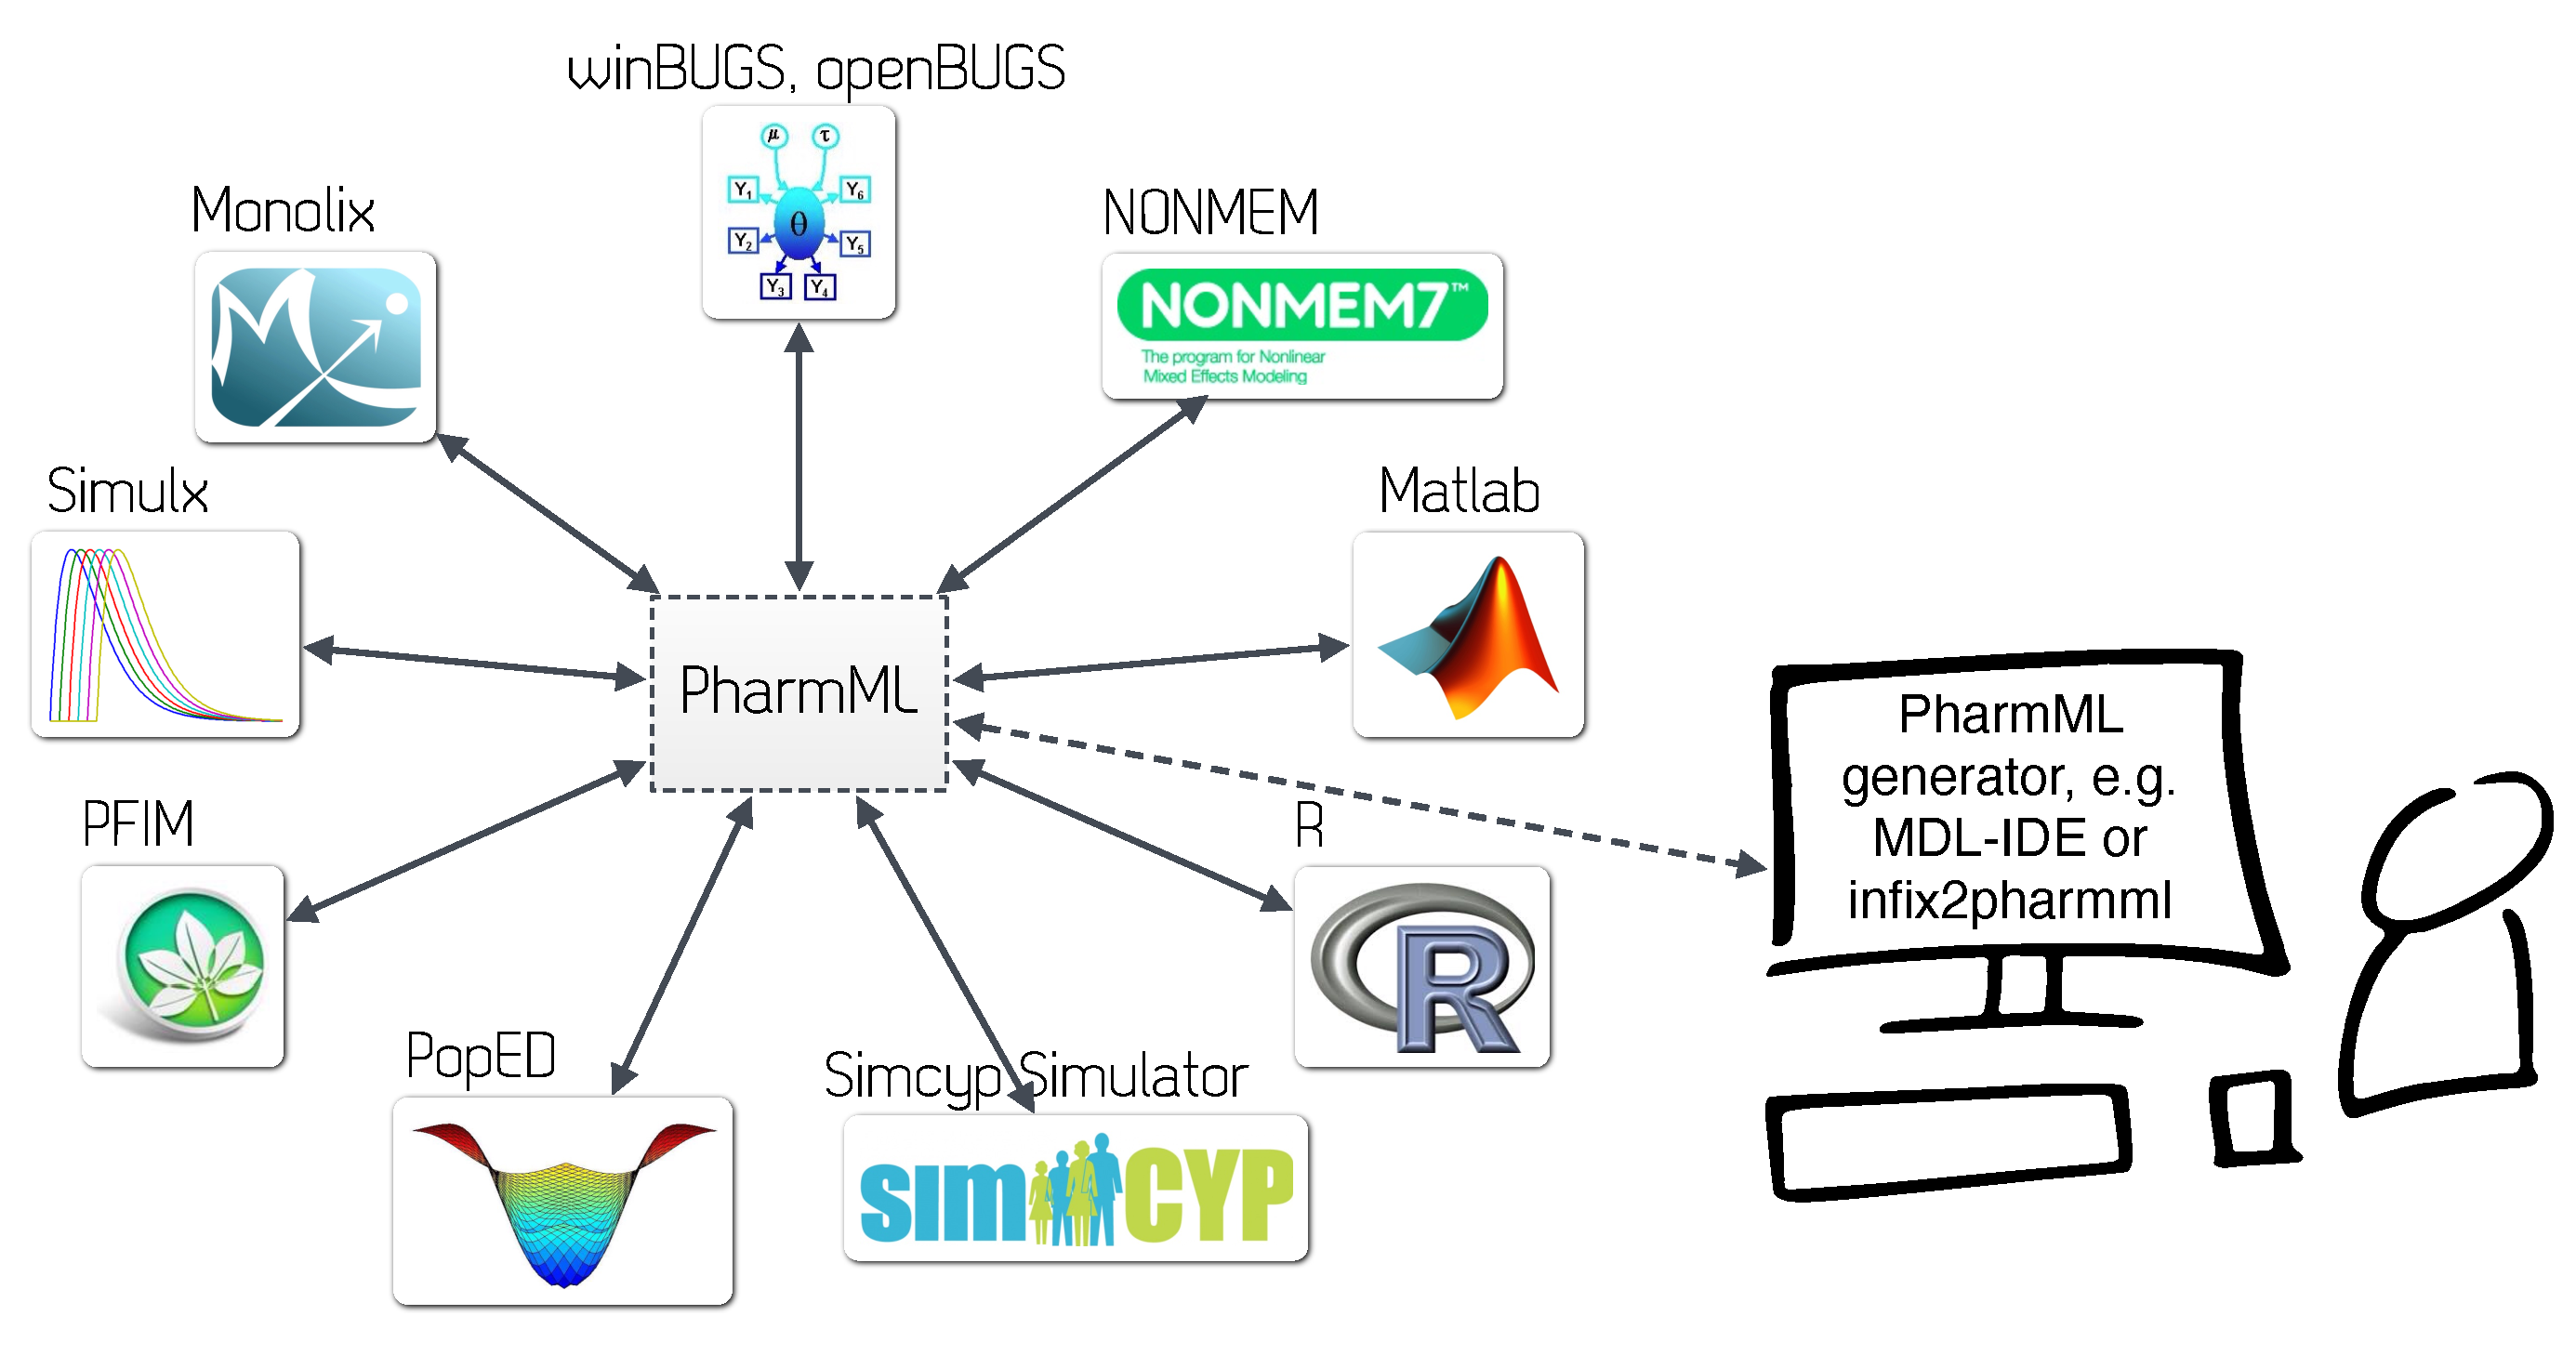
\includegraphics[width=0.95\linewidth]{pics/platformDDMoRe.pdf}
 \caption{Interoperability platform to exchange models via \pharmml.}
 \label{fig:platformDDMoRe}
\end{figure}

This lesson has not been ignored by the pharmacometrics community and in fact a number of years
ago the NLME consortium (a consortium of pharmaceutical companies now all part of \ddmore) started
to work on a very similar standard to \pharmml. This resulted in early drafts of an XML based exchange
language, called PharML, but work on it was unfortunately discontinued and the standard has never been
used and validated. There are a number of other exchange standards in related modelling fields, which we
have drawn on in the development of our work to varying degrees, including:

\begin{description}
\item[CellML] Supports the exchange and storage of computer based mathematical models of 
biological systems \cite{CELLML}.\index{CellML} 
\item[NeuroML] Supports the exchange and description of models ``to describe the biophysics, 
anatomy and network architecture of neuronal systems at multiple scales''\footnote{Quoted 
from \url{http://www.neuroml.org} on 15 Mar 2013.} \cite{NeuroML}.
\item[NineML] Describes neuronal networks in a ``simulator independent 
language''\footnote{Quoted from \url{http://software.incf.org/software/nineml} on 
15 Mar 2013.} that is design to interact with NeuroML \cite{ninemlspec}.
\item[SED-ML] Encodes simulation experiments of SBML and CellML models 
``to ensure exchangeability and reproducibility of simulation 
experiments''\footnote{Quoted from \url{http://sed-ml.org} on 15 Mar 2013.} \cite{sedmll1v1}.
\end{description}

\pharmml is supposed to be the solution in pharmacometrics to the problem. 
An XML based language that will be able to encode models from NONMEM, 
MONOLIX, BUGS and related tools. 
We intend this to be a community standard nucleated around the members of the 
\ddmore consortium. In addition we are developing a software library 
(libPharmML\footnote{\url{https://sourceforge.net/projects/libpharmml.ddmore.p}}) 
to help tool providers incorporate support of \pharmml and to facilitate its
general adoption in the field.

%%%%%%%%%%%%%%%%%%%%%%%%%%%%%%%%%%%%%%%%%%%%%%%%%%%%%%%%%%%%%%%%%%%%%%
\section{The Solution}
\label{intro:objectives}

Having described the problem, we here articulate the \emph{kind} of solution we wanted \pharmml to be.
Developing a language as complex as \pharmml is a difficult undertaking and we wanted to make sure
that we had some firm principles in place to help when designing the language. We've set these aims
and objectives below. \pharmml should:

\begin{description}
%\item[encode models used by pharmacometricians]
\item[describe the mathematics of a model] The language should not include 
information about the authorship of a model, its update history, or the nature 
of the disease process or drug that is being modelled. These aspects will be 
captured by the annotation of the \pharmml document and are out of scope 
of this specification.
\item[describe the task(s) associated with a model] The task(s), such as simulation 
or estimation, to be performed with a model should be encoded in the language.
\item[be declarative] The language should describe \emph{what} information is 
present in a model and \emph{what} the associated task(s) are. It should not 
describe \emph{how} the information is organised, or \emph{how} the task(s) 
should be performed.
\item[be platform independent] Language elements specific to a particular 
modelling tool should not be included. For example it should not describe 
a structural model using a name specific to PREDPP in NONMEM.
\item[serve as an exchange format for the \ddmore infrastructure] The language 
should either support features required by the infrastructure or provide extension 
mechanisms so that additional information can be associated with the \pharmml 
document.
\item[provide support for ontological annotation] The language should provide 
a mechanism for it to be annotated with information that is useful to describe 
the model, but which is beyond the scope of the \pharmml document itself.
\item[enable custom extension] Provide an extensibility mechanism so that 
software tools can associate additional, possibly tool specific information, 
with a \pharmml document.
\item[reuse existing standards where appropriate] Where an established 
information standard exists that can be used to represent information within 
the \pharmml document, we should adopt it.
\end{description}


%%%%%%%%%%%%%%%%%%%%%%%%%%%%%%%%%%%%%%%%%%%%%%%%%%%%%%%%%%%%%%%%%%%%%%
\section{PharmML \& SO -- workflow support and more}\index{workflow}\index{SO}
\label{intro:workflows}
PharmML covers the input for a pharmacometric task, i.e. the model, trail design, 
according task description and experimental data. Another requirements 
posted for our work-package is to provide additionally a structure to store any type
of the numerical results coming from a target tool. This is now an ongoing 
effort and first draft specification of the so called Standardised Output (SO)
is already in use within the framework.

\begin{figure}[ht!]
\centering
  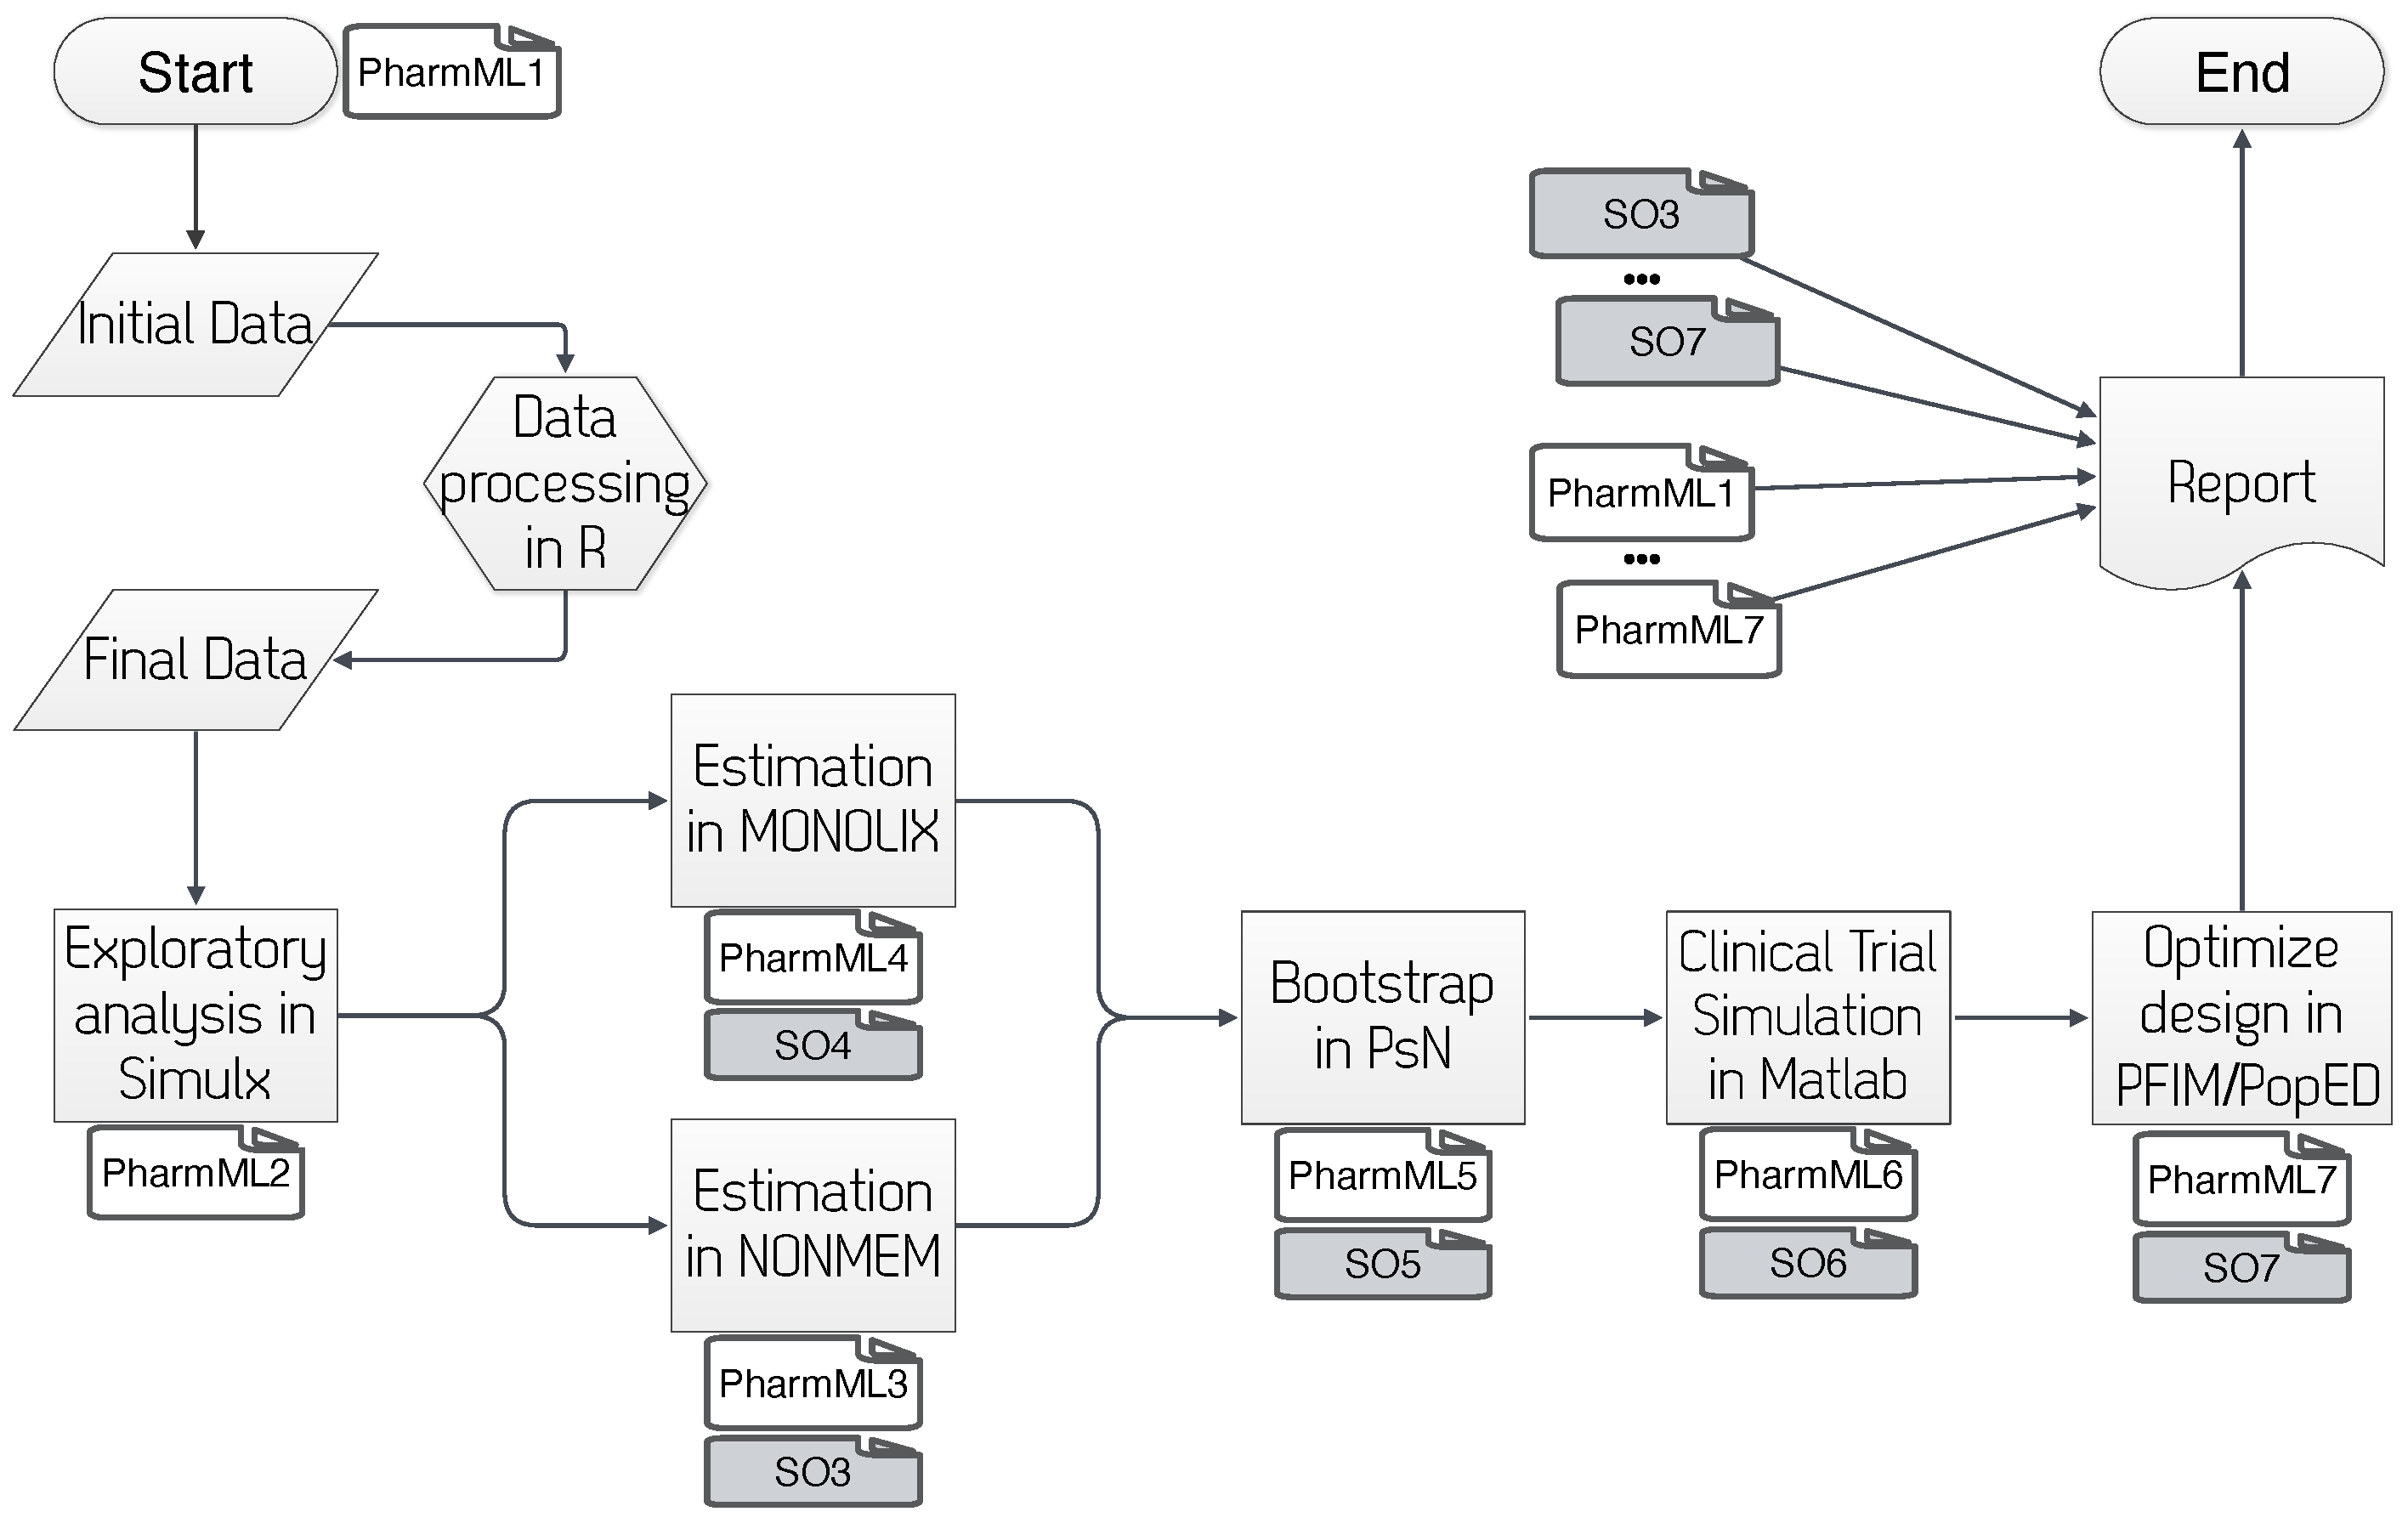
\includegraphics[width=0.95\linewidth]{pics/workflowPharmMLSO}
 \caption{PharmML and Standardised Output (SO) supporting a typical 
 workflow in Pharmacometrics featuring major target tools of the DDMoRe 
 platform. Here, it starts with data processing in R, which can consist of data 
 formatting, merging and/or missing-data imputation. After that an explanatory 
 analysis is carried out in Simulx, followed by estimation using either Monolix 
 or NONMEM. Subsequent steps are bootstrapping using PsN, clinical trial 
 simulation in Matlab and finally Optimal Design in either PFIM or PopED. 
 At every step of the workflow, the PharmML model can be stored and the 
 results following each step can be recorded in the corresponding SO file. 
 Documenting workflows in such a detailed way can potentially simplify 
 reporting and ensures reproducibility.}
 \label{fig:workflowPharmMLSO}
\end{figure}
A first public release of SO is planned in few months. Together, PharmML and SO 
are expected to facilitate:
\begin{itemize}
\item
Smooth and error-free transmission of models between tools
\item
Use of complex workflows via standardised model and output definitions, 
see for an example Figure \ref{fig:workflowPharmMLSO}
\item
Easier reporting and bug tracking
\item
Improved interaction with regulatory agencies regarding modelling and simulation
\item
Reuse of existing model resources, e.g. BioModels database
\item
Development of new tools and methods
\item
Expanding the community developing/applying pharmacometric models.
\end{itemize}

\begin{figure}[ht!]
\centering
  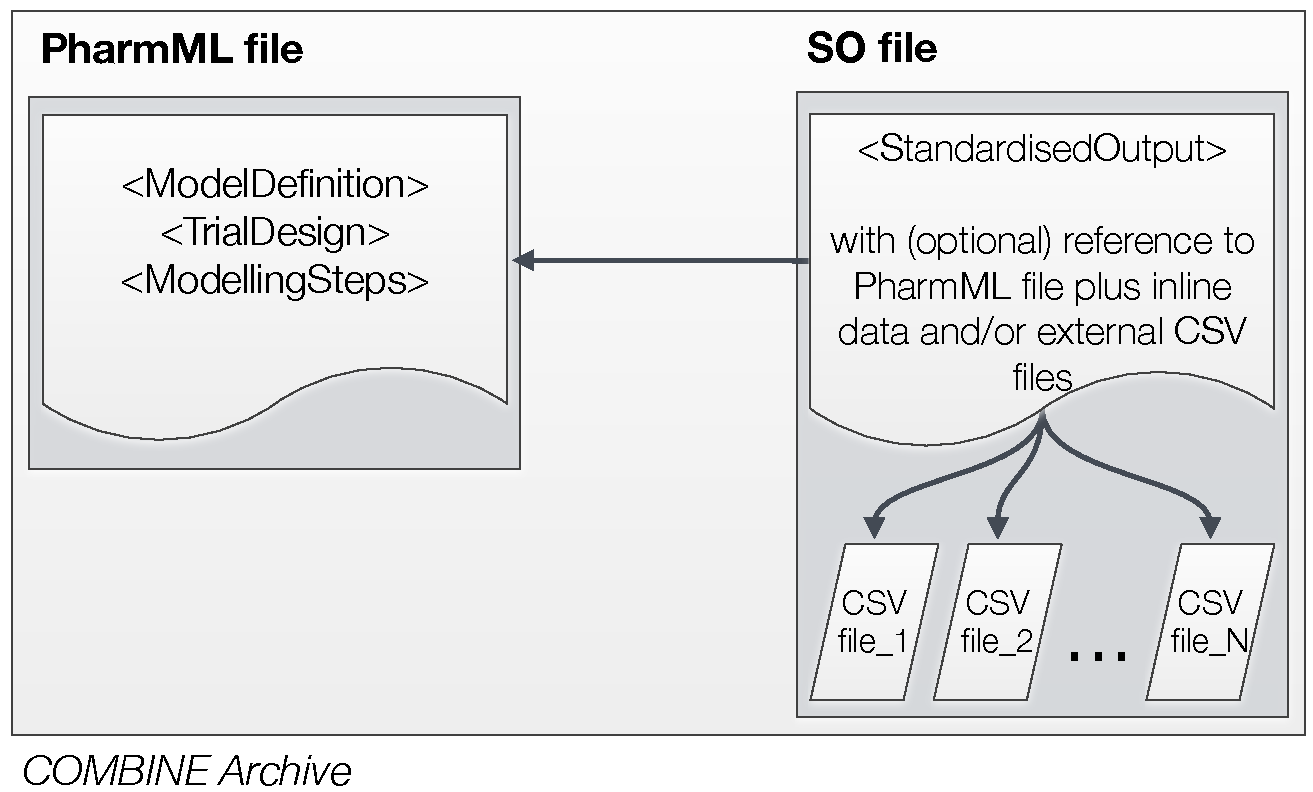
\includegraphics[width=0.6\linewidth]{pics/PharmML_SO}
 \caption{PharmML and Standardised Output (SO) relationship.}
 \label{fig:PharmML_SO}
\end{figure}


%%%%%%%%%%%%%%%%%%%%%%%%%%%%%%%%%%%%%%%%%%%%%%%%%%%%%%%%%%%%%%%%%%%%%%
\section{Creating PharmML coded models}\index{PharmML!editors} 
\label{intro:creatingPharmML}

As indicated in Figure \ref{fig:platformDDMoRe} once a model is encoded 
in PharmML it can be shared with any compatible target tool to perform simulation, 
estimation or optimal design. Modellers will be able in near future to write models 
using a human readable language also developed within DDMoRe, the 
Modelling Description Language, MDL (\url{http://ddmore.eu/mdl}). To facilitate its use, 
an Integrated Development Environment tool, MDL-IDE, is available, within which 
the model is automatically translated to PharmML and can be passed to PharmML 
compatible tools. Development of the MDL and the MDL-IDE is still on-going, 
but initial results are very promising. 

Alternatively, in cases when only the Structural Model is required, modellers can 
already use the web-editor infix2pharmml (\url{http://infix2pharmml.sourceforge.net}) 
to edit complete PharmML models. 


%%%%%%%%%%%%%%%%%%%%%%%%%%%%%%%%%%%%%%%%%%%%%%%%%%%%%%%%%%%%%%%%%%%%%%
\section{The \ddmore Consortium}\index{DDMoRe} 

%Taken from the DDMoRe website need more work.

The Drug Disease Model Resources (DDMoRe) consortium aims to promote collaborative drug and disease
modelling and simulation research. Its aim is to develop tools and standards that will help the
consortium members and later the wider scientific community achieve this goal. Providing \pharmml
is a key goal of the consortium as it underpins a number of related deliverables of the consortium.
In particular:

\begin{itemize}
\item The \ddmore infrastructure in which \pharmml is used to exchange models between the different modelling tools.
\item The \ddmore model repository in which \pharmml will be used to upload and export models to and from the repository. It will also serve as the storage medium for the repository.
\item The \ddmore library of reference models and data-sets, which will provide models in several therapeutic areas. These models will be encoded using \pharmml.
\end{itemize}

The contribution of the \ddmore consortium members in guiding and reviewing the standard has been enormous.
As the standard evolves their role in using and then promoting the standard to the wider community will be invaluable.

Peer review is important in the development of \pharmml and to date we have hosted number of
face-to-face meetings since the development of \pharmml commenced in August 2011. These meetings were:

\begin{itemize}
\item A number of \ddmore consortium meetings in Leiden and Hoofddrop, in the years 2012--2014.
\item The \ddmore technical workshop hosted by Novo Nordisk in Copenhagen, 28--30 Jan 2013.
\item Two \pml technical workshops hosted by University of Pavia, November 2013 \& 2014.
\end{itemize}

\section{How \pharmml was developed}

\pharmml was designed and implemented by a relative small group of individuals, 
but its development has very much been a collaborative process. At the beginning of 
this project we had a number of development guidelines that we adhered to. We aimed to:


\begin{itemize}
\item start with a limited scope and expand the functionality we encode over time.
\item drive development using use cases which reflect the current scope.
\item test the implemented use cases by generating executable models.
\item have frequent review meetings with experts to make sure we are on the right track.
\item use existing technology standards if it is possible and reasonable to do so.
\item use existing information standards if applicable to avoid re-inventing the wheel.
\item make sure the standard is in a form and uses names and terms that make sense to the expert community.
\end{itemize}

In the first half of 2014 an Interoperability Group within the DDMoRe consortium 
was appointed to facilitate the testing of \pml and the interoperability platform driven 
by it. This typically includes 
\begin{itemize}
\item
Creating a MDL coded model in the MDL-IDE (see Figures \ref{fig:platformDDMoRe} 
and \ref{fig:workflowPharmMLSO} for an schematic representation of this and 
the following steps).
\item
Translation from MDL to PharmML.
\item
Translation from PharmML to a target tool language, e.g. MLXTRAN coded model 
for use in Monolix/Simulx or NMTRAN for NONMEM.
\item
Performing a task in a target tool and the export of results into SO.
\end{itemize}
Initial results are very promising, with a number of models being successfully processed 
though this pipeline providing a proof-of-concept for the interoperability concept. 
Figure \ref{fig:DDMoReTimeline} gives an overview of the development timeline, 
more details can be find in the detailed changelog in chapter \ref{cht:changeLog}.

\begin{figure}[ht!]
\centering
  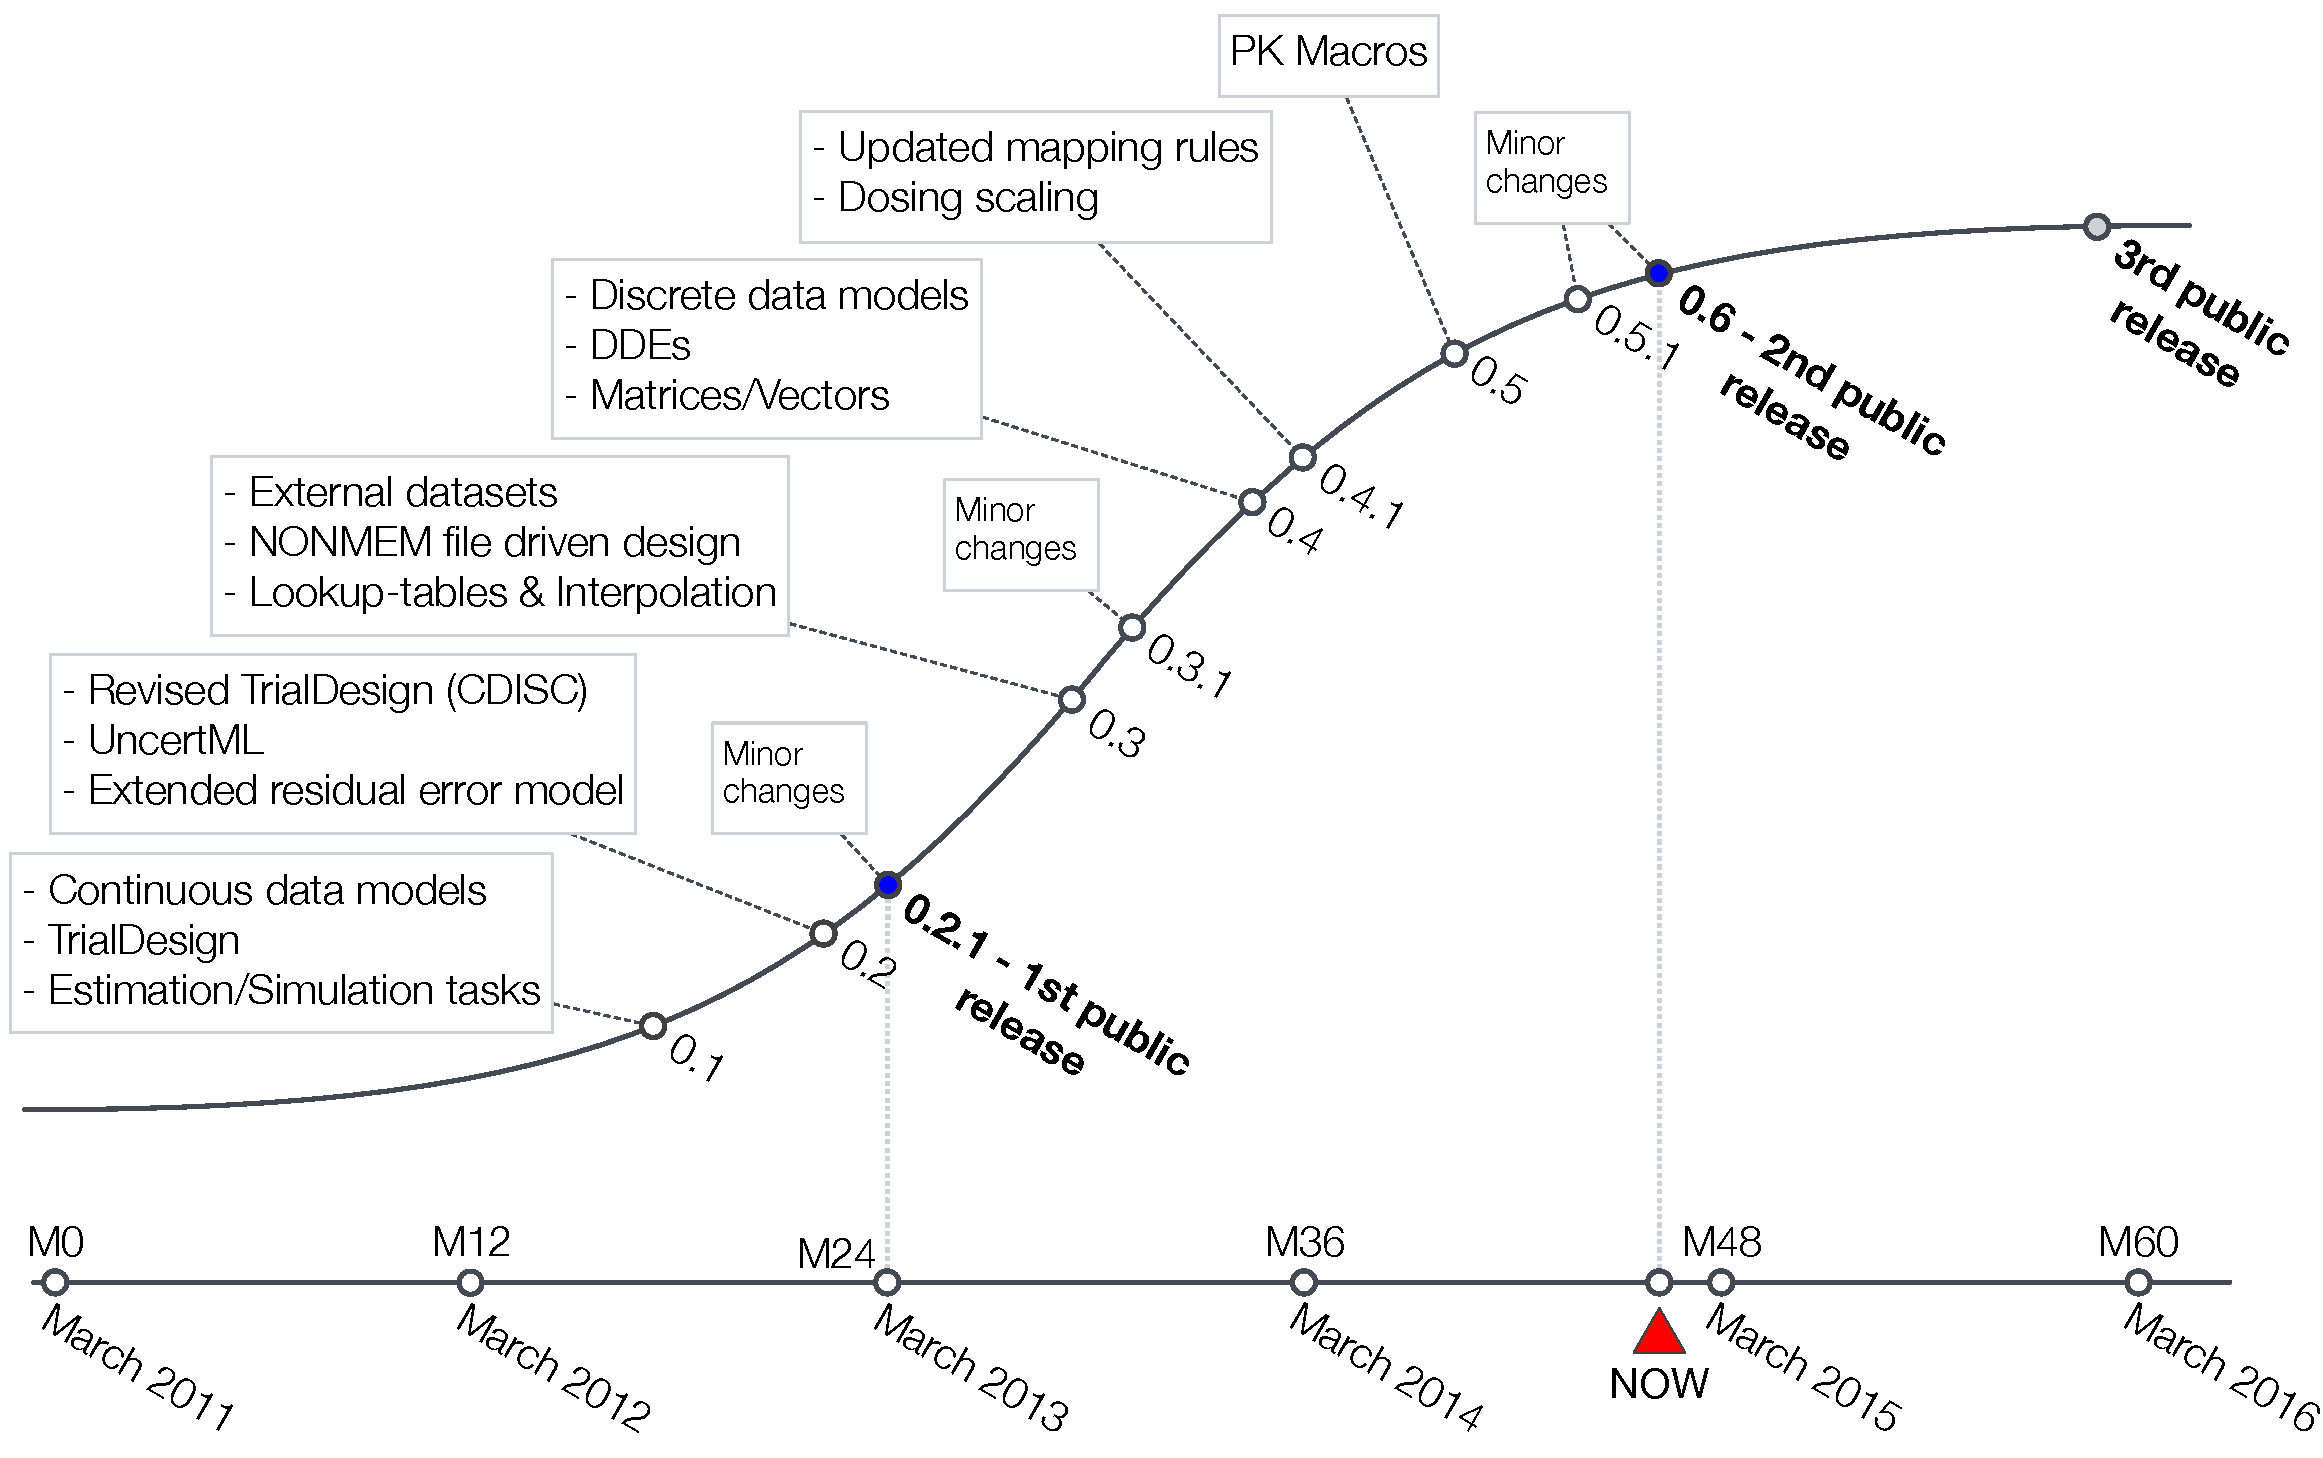
\includegraphics[width=0.95\linewidth]{pics/Timeline.pdf}
 \caption{Timeline of the \pharmml development process, deliverable schedule and version 
 features.}
 \label{fig:DDMoReTimeline}
\end{figure}

\section{Imperative or Declarative?}

In developing \pharmml we have designed it to be a declarative language (see section \ref{intro:objectives}).
While we feel this is the best approach to take for an information exchange langage, it does present us
with number of challenges when dealing with NONMEM, the leading tool in the field. Despite
having a specifically defined language (NM-TRAN \cite{NONMEM:2009}), NONMEM offers a lot of flexibility
to the user, and experienced users can make NONMEM do things that it was never designed to do, to a large
extent because the imperative approach used in NONMEM facilitates this.

The challenge is to convert from the imperative to the declarative language, because there are 
many ways to do the same thing in the imperative language. Therefore, generating 
a \pharmml document from a NONMEM control stream is challenging.

 % It is not the purpose of this document to conduct a detailed comparison between these two approaches but it is important to keep the characteristic differences in mind. One of the main objectives of the DDMoRe project and specifically work-package 4 (WP4) is the building a bridging technology for alternative approaches within one framework. PharmML, the XML based exchange standard which is now available in this first specification is the core element of this interoperability framework.

 % Nevertheless, the differences between these softwares, which manifest themselves mainly in the \emph{imperative} approach of NONMEM versus the \emph{declarative} approach of Monolix, created a chance to a cover broad spectrum of methods and ideas developed over decades. On the one hand FORTRAN-based NONMEM, despite having a specifically defined language (NM-TRAN \cite{NONMEM:2009}), offers almost
 % unlimited flexibility to the user. It can be viewed as a general purpose computational platform and in fact it has been developed
 % as such and can be compared to Matlab or Mathematica (REFs). On the other hand Monolix has been specifically developed for use in pharmacometrics. Although being very flexible, it is based on MLXTRAN, a constantly developing declarative language, defining very precisely the types of allowed models and algorithms.

%Let's put the NONMEM Monolix discussion here and then say that we have adopted a declaritive approach and say why it is better. Need to be careful 
%here to make sure we don't imply that in consequence Monolix is better than NONMEM.

\section{The Evolution of PharmML}
	
This document represents the second public release of \pharmml. The first one was released  
on 21$^{st}$ November, 2013, \cite{Pharmml_021}.

Any piece of software is upgraded as users request new features and developers find better 
ways to do the same thing. A successful standard is no different and with success in mind we 
expect \pharmml to evolve and change further as it is subject to the same influences. To manage this 
process we have adopted the following strategy to record versions of the \pharmml specification.

\paragraph{Version number}\index{PharmML!release version} 
\label{intro:versioning}

To record changes in the specification we will use the following three level numbering system, of the form
$x.y.z$. The levels correspond to the following types of revision:

\begin{description}
\item[$x$ major] Significant new features or radical change of design.
\item[$y$ minor] New features or evolutionary design changes.
\item[$z$ patch] Error corrections.
\end{description}


%%%%%%%%%%%%%%%%%%%%%%%%%%%%%%%%%%%%%%%%%%%%%%%%%%%%%%%%%%%%%%%%%%%%%%
\section{Feedback}\index{PharmML!related websites} 

User and developer feedback is important. Typically,
this feedback will be in the form of a specific issue: either to report defects identified in
the specification or to request new features. Either way the specific issues can be submitted
to the tracker at: \url{https://github.com/pharmml/pharmml-spec/issues}. In some cases it is practical to raise
an issue that is broader than a specific issue or requires some discussion within the community. 
Here the contact is the \pharmml forum at \url{http://pharmml.org}.
